% !TEX root = ../Report.tex

In this section an detailed description of the dataset will be given. The process of data preprocessing and the training process for both architectures will explained.

\subsection{LUNA16 dataset}

The used dataset is from the LUNA16 challenge and each scan contains a number of slices. The algorithm creates a label map for each slice marking every pixel that is part of the lung. An example of one scan and the corresponding labeling is shown in figure \ref{scan_picture}.

\begin{figure}[h!]
	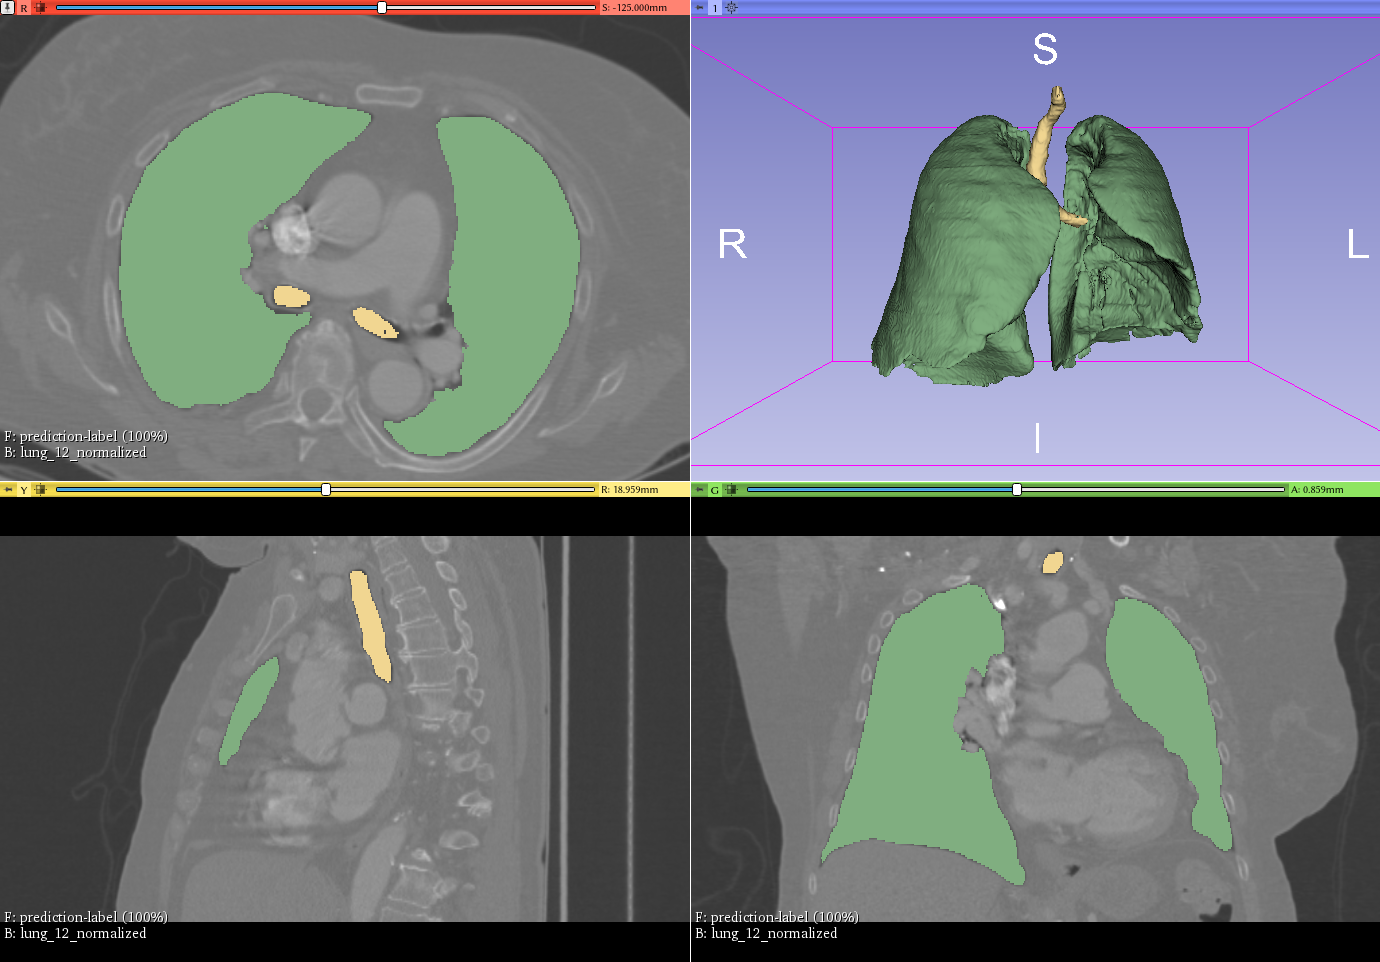
\includegraphics[width=0.49\textwidth, angle=0]{files/Fulllayoutprediction.png}
	\caption{CT scan of the lung and labeled lung (green) and the tube (yellow). The first picture represents one slice of the image, the second a 3D representation of the label and the lower two pictures are visualizations of the side and front view.}
	\label{scan_picture}
\end{figure}

The dataset consists of about 10 GB of mdh and raw image files. The files contain a varying number of slices of 512 x 512 pixel grey-scale images and corresponding 512 x 512 pixel label maps. Since computational resources were limited just a subset of the data was used for this work. Furthermore the more detailed label map was reduced to one label for the lungs and one label for the bronchus.\newline
From the LUNA16 dataset 10 CT scans for training and 20 CT scans for evaluation were chosen randomly.

\subsection{Preprocessing of image data}
Each file was converted to a NIfTI image file for better processing and visualization. These files contain all grey-scale image slices of one scan. For more appropriate input values, each image was normalized following the standard normal distribution ($\mu = 0.0$ and $\sigma = 1.0$) separately.\newline
Then, it was necessary to implement data importation to properly use them. Data from directory were converted into input and label matrices following the size 512x512 for each slice (on average 200 slices per image).

\subsection{Training and validation}
Both network architectures were trained on the 2145 slices of the 10 training CT scans over 35 epochs.\newline
For the DeepMedic architecture a open-source implementation \cite{deepmedic} was modified for the purpose of lung segmentation and the parameters were set up according to successful implementations for brain tumor detection. RMS propagation with a initial learning rate of 0.001, the Nesterov momentum (momentum rate of 0.06) and L2 regularization (regularization rate of 0.0001) were used as an optimizer. For the training a batch size of 10 samples was chosen and the network was evaluated with the binary cross entropy (BCE) as a loss function.\newline
The U-Net architecture was built up according to the structure in figure \ref{unetstructure}. For the training process the Adam optimizer with the described loss function $Loss = dice loss + BCE$ from chapter \ref{metrics_chapter} was used in combination with a batch size of 3 slices. To get an idea of the performance of the model during training 10 \% of the slices were used for validation in each epoch.\newline

\subsection{Dealing with the big dataset}
Although the dataset was reduced to 10 CT scans some adjustment in the training process still had to be made to handle the size of the dataset.\newline
Therefore, a generator was defined to reduce the data size that will be fed to the training process at once. The generator feeds just a batch of images in real time to the training process instead of loading the whole dataset at once.